\subsection{Installatie}
De installatie van OctoberCMS kan op twee manieren. Clone via Github het project of download een installer pakket. De eenvoudigste manier van installatie is via de installer te werken. Deze manier levert hetzelfde resultaat op, echter met een minimum aan inspanning. Start een lokale server op en maak een database aan. Zorg ervoor dat je over de nodige rechten beschikt vooraleer de installatie van start te laten gaan. Dit kan anders problemen geven bij de connectie van de database. Via de install.php file in de browser wordt je begeleid door de installatie van OctoberCMS. Via deze stapsgewijze configuratie is het CMS in geen tijd geïnstalleerd en klaar voor gebruik. 
\newline\newline
Een belangrijke configuratie om in acht te namen is de opbouw van de site. Er zijn namelijk drie manieren om de site te configureren. De minst vooraf geconfigureerde optie is te starten van 'scratch'. Deze optie wordt geïnstalleerd met een basis thema dat minimale opmaak heeft. Een demo plugin zorgt voor wat opvulling van de site. Een tweede mogelijkheid is te kiezen voor vooraf geconfigureerd thema met daar bijhorende plugins. Deze optie is een goed startpunt om OctoberCMS te leren kennen of om snel een blog of portfoliosite op te stellen. De laatste optie is te kiezen om een bestaand project te importeren. Handig indien je bestaande plugins en thema's wil importeren vanaf de installatie.

\begin{figure}[!ht]
  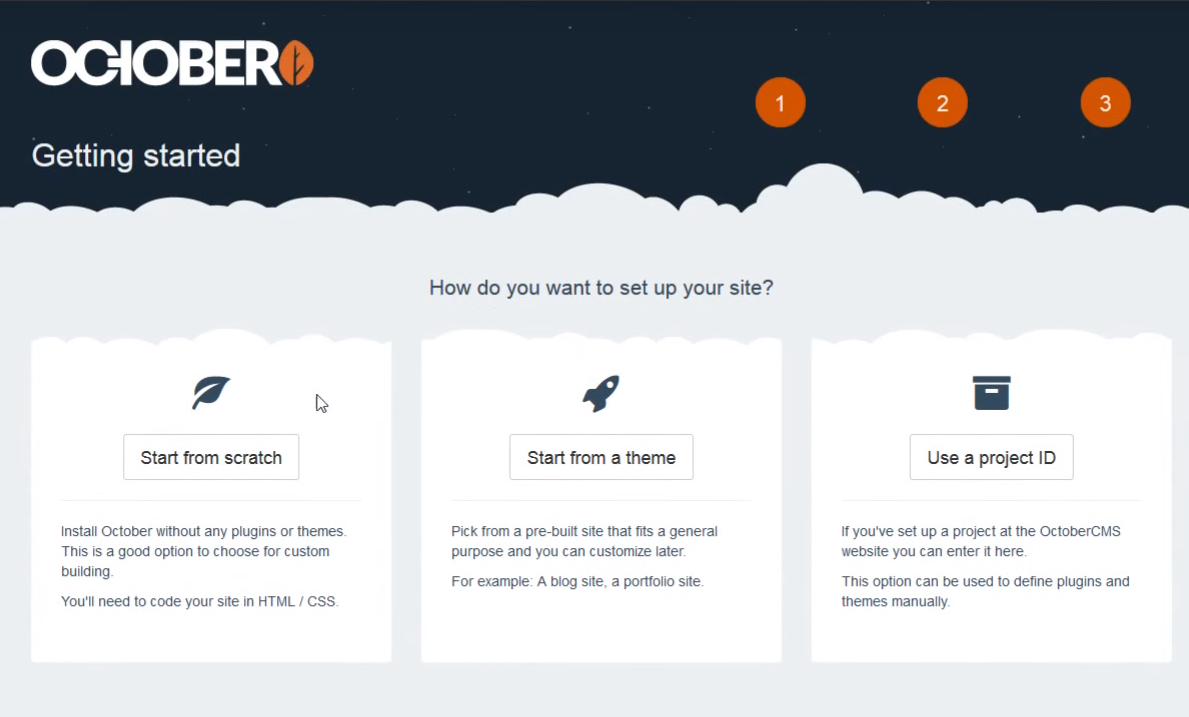
\includegraphics[width=120mm]{img/octobercms-configuration.png}
  \centering
  \caption{OctoberCMS site configuratie}
  \label{fig:OctoberCMS site configuratie}
\end{figure}

\noindent
Als ontwikkelaar is het in de meeste gevallen de beste optie om te kiezen om te starten van 'scratch'. Hierbij wordt er gestart van een 'schone lei' en bevat de installatie enkel code die nodig is. 
\newline\newline
Nadat de installatie is afgerond, is het belangrijk om veiligheidsredenen de installatiebestanden te verwijderen. 
\newline\newline
Het doorlopen van de installatie neemt hooguit 5 minuten in beslag. Het doorlopen van dit proces kan gestaafd worden aan de hand van volgende screencast \citep{LearnTogether2016InstallXAMPP}.


\subsection{Theming}
Een thema is de basis van output naar de gebruiker toe. Elk thema bevat verschillende sub folders die de website zijn huidige look en feel zal geven. Een standaard installatie bevat een bestaand thema. Dit thema later kan worden overschreven of vervangen kan worden door een eigen thema. Er kan eenvoudigweg van thema worden geswitcht via de back-end in de browser of door de 'activeTheme' instelling aan te passen in het cms.php bestand. Dit bestand is terug te vinden in de 'config' folder. De opbouw van een thema ziet er als volgt uit:

\begin{figure}[!ht]
  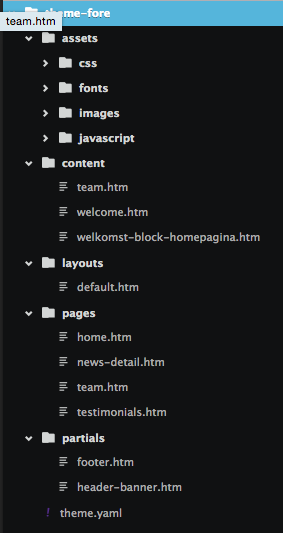
\includegraphics[width=50mm]{img/folder-structure.png}
  \centering
  \caption{OctoberCMS folder structuur}
  \label{fig:OctoberCMS folder structuur}
\end{figure}

\pagebreak
\noindent
Elk thema heeft sub folders voor assets, content, layouts, pages en partials. Het theme.yaml bestand bevat de thema configuratie. Zaken als naam, omschrijving, auteur en code van het thema, worden in dit bestand beschreven. Bestanden krijgen de extensie .htm en maken gebruik van Twig markup. Twig is één van de vele PHP template engines. Twig richt zich op propere en overzichtelijke code en wordt bij het uitvoeren omgezet in geoptimaliseerde PHP code. 
\newline\newline
Elke template pagina kan bestaan uit drie onderdelen. Een blok voor configuratie, PHP code en Twig code. Elk van deze blokken worden van elkaar onderscheiden door twee '=' symbolen.  De configuratieblok bestaat uit een route of URL naam en een eventuele layout template. Een layout template specificeert de layout van een pagina. Deze pagina zorgt ervoor dat gelijke stukken code die over verschillende pagina's heen gebruikt worden, slechts één keer aangemaakt moeten worden. Het PHP code blok is optioneel en bevat functies die steeds uitgevoerd worden alvorens de pagina gerenderd wordt. Deze code wordt omgezet naar een aparte PHP file bij het compileren. Het derde blok bevat de Twig markup code die gerenderd en gecompileerd wordt naar html in de browser. Het Twig gedeelte bevat alle code die de zichtbare elementen op de pagina zullen weergeven aan de gebruiker.

\begin{figure}[!ht]
  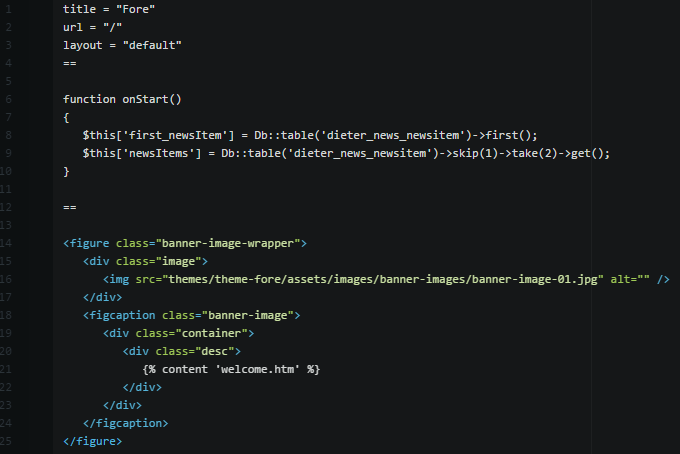
\includegraphics[width=\textwidth]{img/screen-homepage.png}
  \centering
  \caption{Home template pagina}
  \label{fig:Home template pagina}
\end{figure}

\noindent
Naast een layout template onderscheiden we ook partials. Herbruikbare elementen die beschreven worden in een aparte pagina. Deze kunnen toegevoegd worden aan andere pagina's. Vaak voorkomende elementen die in een partial worden gestopt zijn een footer en header. Het toevoegen van een partial op een pagina is eenvoudig. Roep via de Twig annotatie de partial op en de daarbij horende bestandsnaam. Er wordt automatisch gezocht in de partial folder van het thema naar de bestandsnaam. 

\begin{figure}[!ht]
  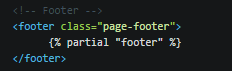
\includegraphics[width=75mm]{img/partial-impl.png}
  \centering
  \caption{Partial implementatie}
  \label{fig:Partial implementatie}
\end{figure}

\noindent
Content blocks bevatten een statische inhoud en kunnen bestaan uit tekst, HTML of Markdown. Markdown is een bestandstype dat tekst zonder opmaak bevat en wordt omgezet naar HTML \citep{GruberJohn2004Markdown}. Een content block kan onafhankelijk van de de pagina waarin het is toegevoegd, veranderd worden. Een content sectie kan heel eenvoudig door de eindgebruiker in de back-end van de browser aangeroepen en aangepast worden. Een content block kan op twee manieren worden aangemaakt. Ofwel via de back-end van de browser, ofwel door een .htm document aan te maken in de 'content' folder van het thema. 
\newline\newline
De folder met assets kan allerhande subfolders en documenten bevatten. De standaard opbouw van een assets map bevat een folder voor alle CSS documenten, een images folder voor alle gebruikte afbeeldingen en een javascript folder als verzamelmap voor alle script documenten.

\subsection{Menu en routing}
\subsubsection{Routing}

Routing in OctoberCMS is opgesplitst in een routing voor back-end controllers en CMS pagina's. De routing van de back-end controllers gebeurt afzonderlijk per plugin. Plugins worden hieronder uitgebreid besproken. Daarom is het momenteel voldoende te weten dat de controller klasse communiceert met de views pagina's via de naam toegewezen aan de views pagina. De routing voor de standaard pagina's index, create, preview en update gebeuren automatisch. Het is uiteraard mogelijk deze automatische routing te overschrijven.
\newline\newline
De routing van de CMS pagina's zit logisch en eenvoudig in elkaar. Een pagina krijgt een URL toegewezen in het configuratie gedeelte van elke pagina. Elke pagina URL wordt voorafgegaan door een slash (/). Het voorbeeld hieronder weergegeven is de meest eenvoudige vorm van routing.

\begin{figure}[!ht]
  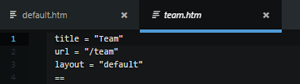
\includegraphics[width=75mm]{img/oc-routing-url.png}
  \centering
  \caption{URL routing}
  \label{fig:Url routing}
\end{figure}

\noindent
Het is mogelijk om een URL op te bouwen aan de hand van bijgevoegde parameters. Deze parameters worden aangeroepen in de PHP sectie van de pagina. Op deze manier kan de pagina dynamisch aangemaakt worden afhankelijk van de waarde van de parameter. Een parameter kan optioneel zijn wanneer die zich op het einde van de URL bevindt. Een optionele parameter wordt aangegeven via een vraagteken achter de parameter.

\begin{figure}[!ht]
  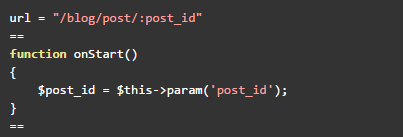
\includegraphics[width=75mm]{img/oc-routing-url-parameter.png}
  \centering
  \caption{URL routing met parameter}
  \label{fig:Url routing met parameter}
  \citep{BobkovAlexey2016OctoberCMSDocumentation}
\end{figure}


\subsubsection{Menu}
In de meeste gevallen is een menu een statisch gegeven. Menu items behoren niet tot de dagelijkse aanpassingen van een site. OctoberCMS opteert dan ook standaard een menu statisch te implementeren. Een menu wordt het beste rechtstreeks in de layout pagina gezet of aangemaakt als partial.
\newline\newline
Twig beschikt over tags, filters en variabelen die aangeroepen kunnen worden binnen een pagina. Bij het linken van een pagina gebruik je de '|page' filter. Deze filter maakt een link gebruikmakend van de pagina naam. De gegeven naam linkt naar de opgegeven URL in het configuratie gedeelte van de pagina (zie Routing). 

\pagebreak

\begin{figure}[!ht]
  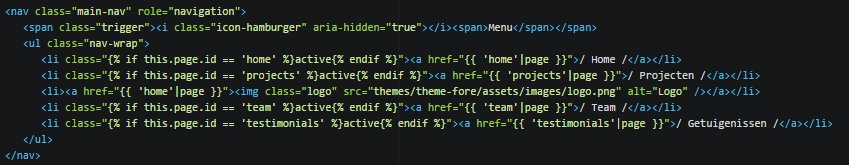
\includegraphics[width=\textwidth]{img/oc-menu.png}
  \centering
  \caption{Code voor het menu, geïmplementeerd in de layout pagina.}
  \label{fig:Menu}
\end{figure}

\noindent
Het is mogelijk een vaste parameter door te geven aan de link om bijvoorbeeld te linken naar een post met bepaalde ID. Parameters worden tussen haken na de '|page' filter geplaatst.

\begin{figure}[!ht]
  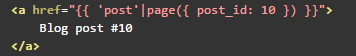
\includegraphics[width=75mm]{img/oc-menu-parameter.png}
  \centering
  \caption{Menu met parameter}
  \label{fig:Menu met parameter}
  \citep{BobkovAlexey2016OctoberCMSDocumentation}
\end{figure}

\noindent
Voor gevallen waarbij een menu aanpasbaar moet zijn voor de eindgebruiker heeft OctoberCMS een oplossing geboden. Een plugin genaamd MenuManager zorgt ervoor dat het managen van uw menu in de back-end via de browser kan beheerd worden. Omdat dit eerder een specifiek en minder voorkomend gebeuren is, wordt dit niet verder getest en besproken.

\subsection{Plugins en modules}
Plugins kunnen gezien worden als de belangrijkste elementen voor het uitbreiden van OctoberCMS. Elke plugin komt in de map '/plugins' en heeft een vaste mappenstructuur. Een plugin kan verschillende elementen definiëren. Back-end pagina's en menu's, interactie met andere Plugins, components, enz.

\subsubsection{Organisatie Plugins}

\textit{Overzicht} \newline
Standaard wordt bij een installatie van OctoberCMS, ook bij een installatie 'from scratch', een plugin geïnstalleerd. Deze plugin doet enkel dienst als demo. Een overzicht van alle geïnstalleerde plugins kan je zien aan de hand van je mappenstructuur. De visuele weergave in de back-end van de browser biedt meer overzicht. Een oplijsting in tabelvorm waarbij je alle plugins met hun belangrijkste informatie kan bekijken. Deze lijst is terug te vinden op de Update pagina onder instellingen. 

\begin{figure}[!ht]
  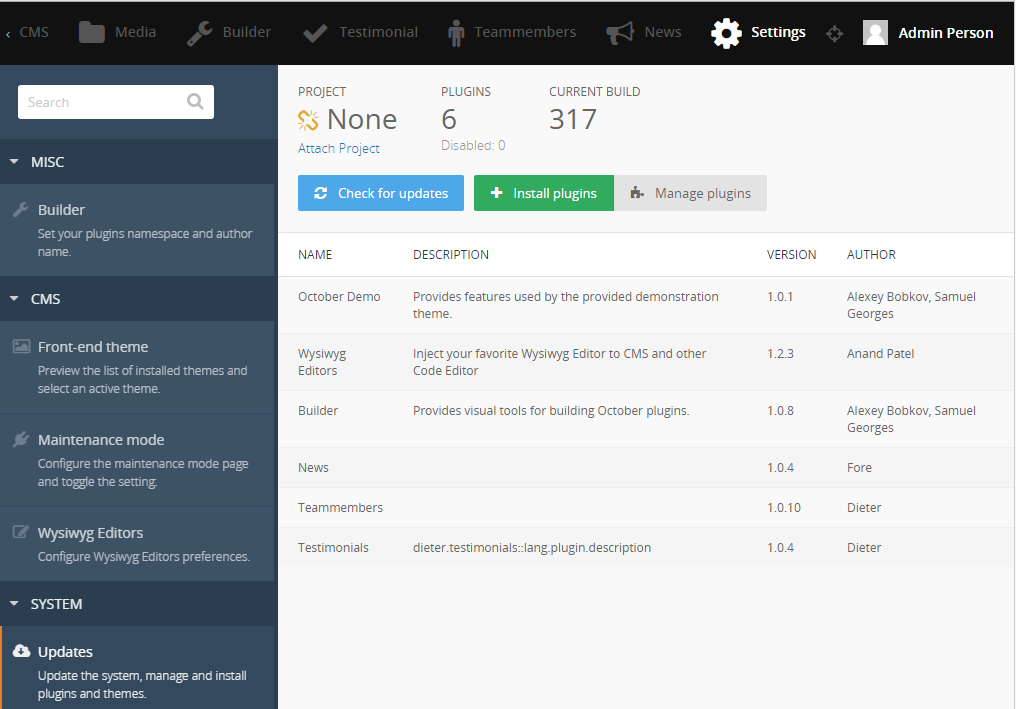
\includegraphics[width=\linewidth]{img/oc-plugin-updates.png}
  \caption{Overzicht geïnstalleerde plugins}
  \label{fig:Overzicht geïnstalleerde plugins}
\end{figure}

\pagebreak
\noindent
\textit{Marketplace}\newline
De Marketplace van OctoberCMS is een opslagplaats van alle gepubliceerde plugins en thema's. Elke ontwikkelaar kan zich registeren op de Marketplace en op die manier thema's en plugins publiceren. Bij het publiceren van een plugin of thema wordt deze eerst gescreend en onderworpen aan testen die op zoek gaan naar bugs of fouten. Een publicatie kan je gratis of tegen betaling ter beschikking stellen. De Marketplace is een groeiend platform waar er momenteel 317 plugins te verkrijgen zijn (geraadpleegd op 05/05/2016). Als ontwikkelaar kan je ook een aardig centje bijverdienen indien je plugin goed gebouwd en een nuttige aanvulling is. Als we kijken naar statistieken die te raadplegen zijn op de Marketplace, zien we een klein overzicht van de populairste plugins, thema's en auteurs.

\begin{figure}[!ht]
  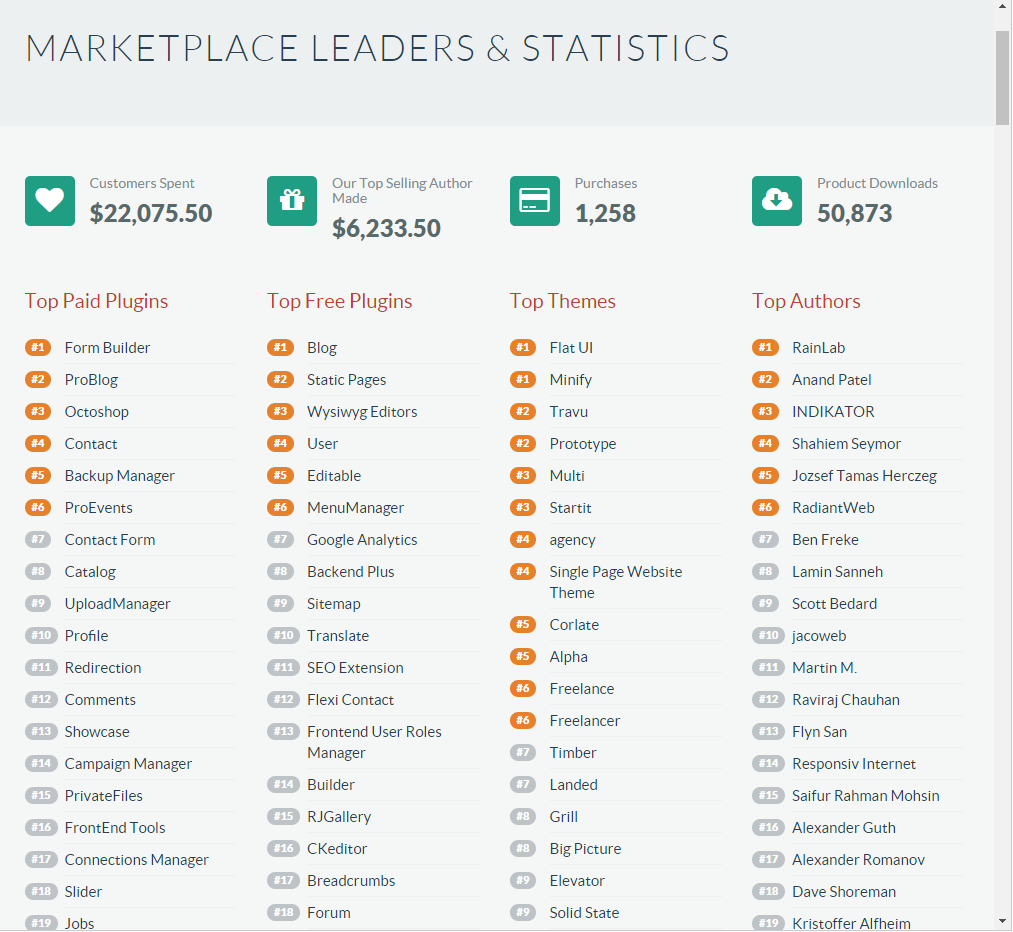
\includegraphics[width=\linewidth]{img/oc-marketplace-plugins.png}
  \caption{Overzicht populaire plugins, thema's en auteurs op de MarketPlace (geraadpleegd op 05/05/2016).}
  \label{fig:Overzicht populaire plugins, thema's en auteurs op de MarketPlace}
\end{figure}

\pagebreak

\noindent
\textit{Installeren}\newline
Alvorens een plugin te installeren dien je eerst een project aan te maken op je account in OctoberCMS. Dit project kan je koppelen met een unieke sleutel aan je site. Dit proces doorlopen is niet nodig wanneer je lokaal werkt.
\newline\newline
Installeren van een bestaande gratis plugin kan vanuit de site zelf. Via de knop 'Install Plugins' is het mogelijk om plugins te zoeken en te installeren die gestockeerd zijn op de Marketplace. Plugins die betalend zijn moeten eerst aangekocht worden. Achteraf kunnen deze worden toegevoegd aan een project. 
\newline\newline
\noindent\textit{Ontwikkelen}\newline
Naast de vele plugins die te vinden zijn op de Marketplace kan het voorkomen dat iets 'custom built' moet gemaakt worden. Wanneer beschikbare plugins niet voldoen aan de wensen van de klant, moet een nieuwe plugin ontwikkeld worden. 
\newline\newline
Ontwikkelen van een nieuwe plugin kan op drie manieren aangepakt worden. Elke plugin wordt in een folder aangemaakt met een unieke auteursnaam.
\newline\newline
Een plugin kan volledig manueel aangemaakt worden. Dit is de meest arbeidsintensieve manier en zeker niet de eenvoudigste. Hierbij maak je elke file manueel aan met de daarbij horende code. Een interessantere manier is te werken via de command-line-interface die gebruikt wordt bij Laravel. Artisan bevat een lijst met handige commando's die het ontwikkelen eenvoudiger en sneller maakt. Het aanmaken van een plugin met een standaard opmaak van folders en files gaat eenvoudig via volgend commando:

\begin{minted}{c}
	php artisan create:plugin dieter.teammembers
\end{minted}

\noindent
Hierbij wordt een upgrades folder aangemaakt met een version.yaml bestand. Deze folder en file houden de veranderingen van de plugin bij. Daarnaast hebben we een bestand Plugin.php waarin de algemene configuratie van de plugin in vermeld staat. Een plugin kan verder opgebouwd worden met models-, controllers-, language-, en classes folders, afhankelijk van de functie van een plugin. 
\newline\newline
Het aanmaken van deze mappen en files kunnen allemaal via Artisan. Artisan biedt commando's voor elk van deze opdrachten. 
\newline\newline
De laatste manier om een plugin aan te maken en te configureren is via een bestaande plugin. De Builder plugin is een relatief nieuwe plugin die gelanceerd is op 10 februari 2016 door de makers (Rainlab) zelf. Het verkort en vereenvoudigt het ontwikkelen van een plugin. Het is een ideale manier om een plugin snel op te zetten en achteraf aanpassingen te doen in code of via de Back-end in de browser. De Builder plugin is ontwikkeld om de repetitieve activiteiten te automatiseren zonder de controle te verliezen. Op deze manier is er meer tijd vrij voor de belangrijkere business logica. 
\newline\newline
Via een chronologische structuur van de Builder plugin doorloop je de verschillende stappen en heb je in geen tijd een tabel opgebouwd die gelinkt is aan een model. Controllers geven je de mogelijkheid data in te voeren en te beheren. Het invoeren gaat via een formulier. Het beheren en visualiseren is via een lijst. Beide controllers kunnen volledig geconfigureerd worden. Op ieder moment is het mogelijk om te schakelen naar een editor om de nodige aanpassingen te doen in code.

\begin{figure}[!ht]
  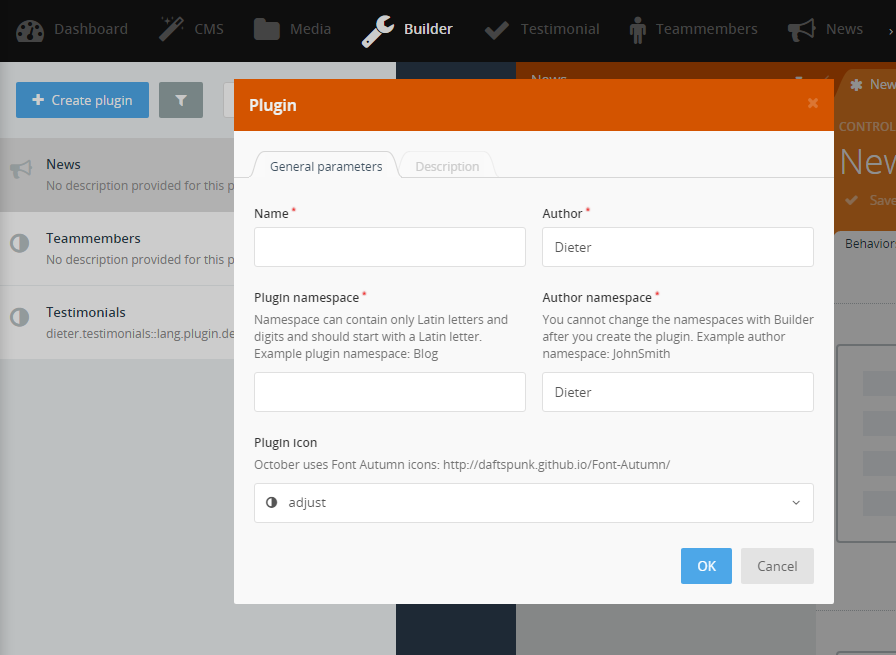
\includegraphics[width=\textwidth]{img/oc-builder-create.png}
  \caption{Het aanmaken van een nieuwe plugin via de Builder plugin is eenvoudig. Via het pop-up venster geef je een unieke naam en de auteur in. Personaliseer met een icoon.}
  \label{fig:Builder Plugin, Plugin aanmaken}
\end{figure}

\begin{figure}[!ht]
  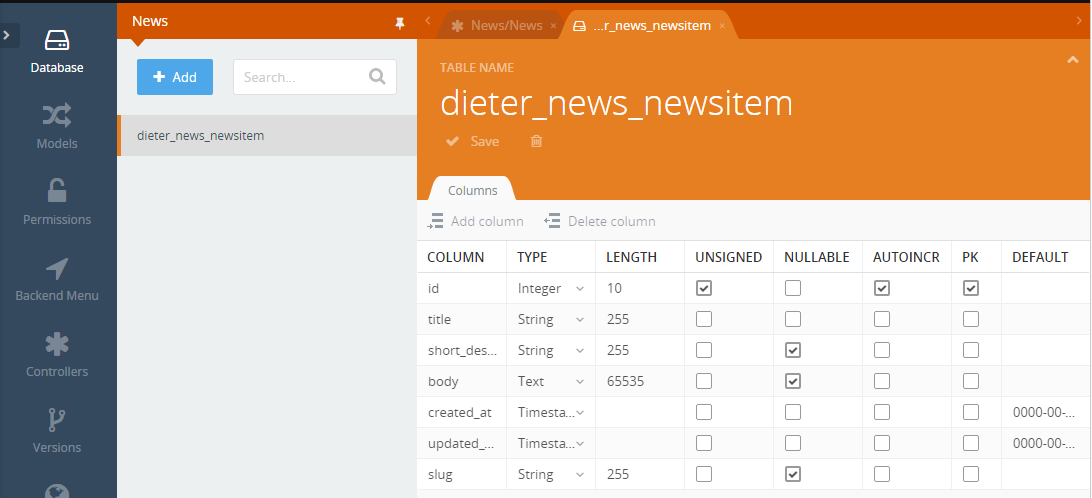
\includegraphics[width=140mm]{img/oc-builder-db.png}
  \centering
  \caption{Maak via de tabel de nodige kolommen aan. Eenmaal opgeslagen wordt een query uitgevoerd op de database.}
  \label{fig:Builder Plugin, Database tabel aanmaken}
\end{figure}

\begin{figure}[!ht]
  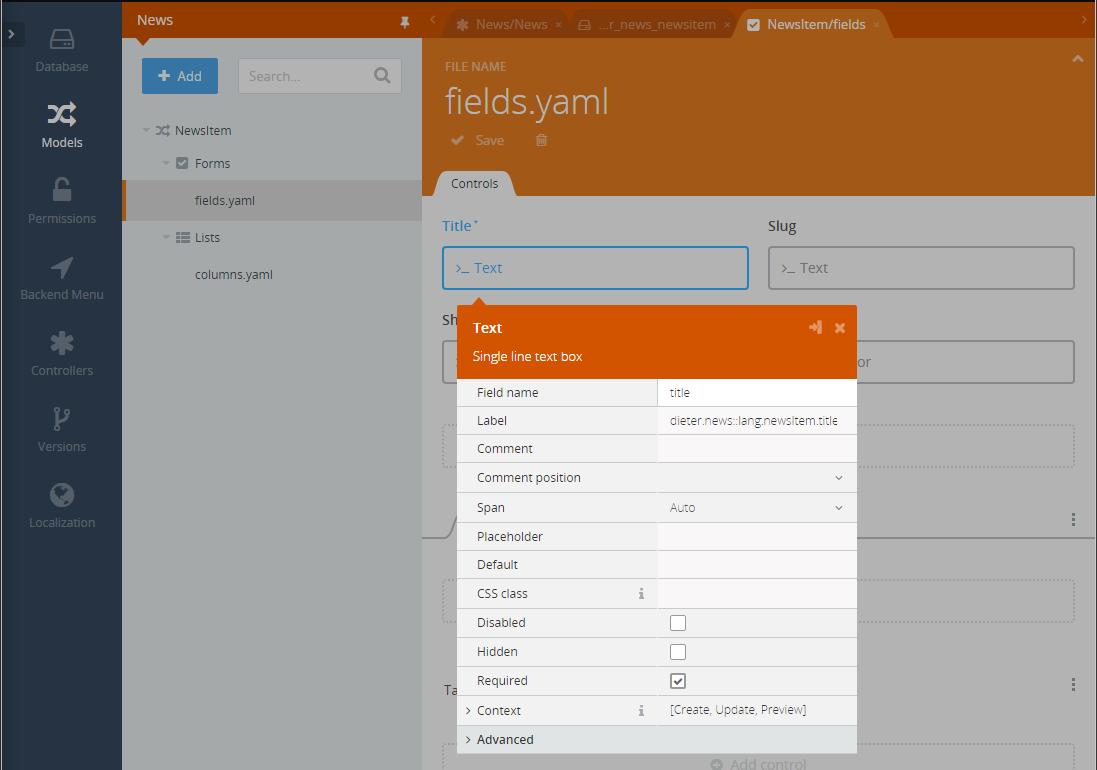
\includegraphics[width=140mm]{img/oc-builder-model.png}
  \centering
  \caption{Configureer een model. Vul de nodige velden aan en link ze met tabelnaam uit de database. Configureer waar nodig.}
  \label{fig:Builder plugin, model aanmaken}
\end{figure}

\begin{figure}[!ht]
  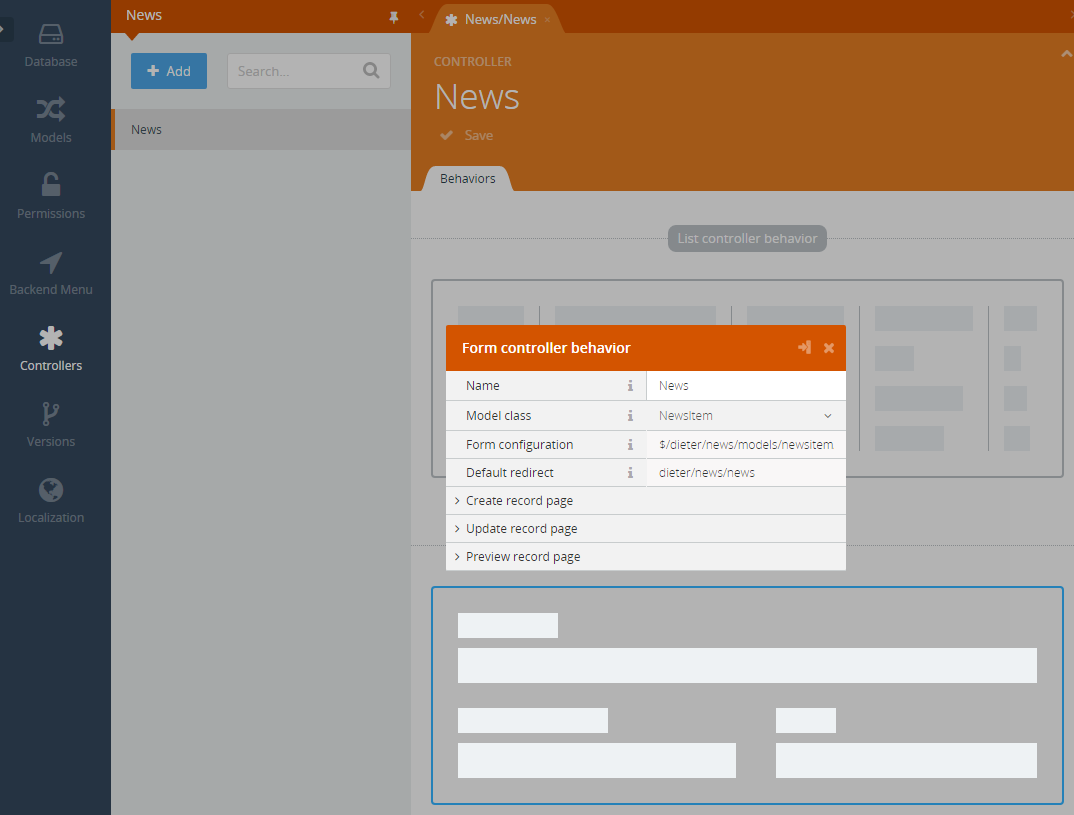
\includegraphics[width=140mm]{img/oc-builder-controller.png}
  \centering
  \caption{Configureer en link de models aan de controller klasse. }
  \label{fig:Builder plugin, controller aanmaken}
\end{figure}

\pagebreak
\noindent
De Builder plugin biedt ook een permissie systeem waarbij de toegang wordt beschreven voor verschillende gebruikers of gebruikersgroepen. De tab back-end menu laat je toe de plugin weer te geven bovenaan de taakbalk. Een menu kan bestaan uit verschillende sub items.
\clearpage
\noindent
Wanneer het volledige proces van de Builder plugin doorlopen is, verkrijgen we bijvoorbeeld volgende mappenstructuur: 

\begin{figure}[!ht]
  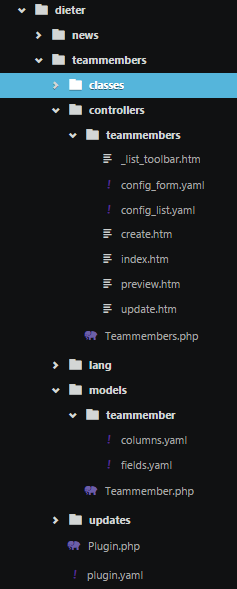
\includegraphics[width=50mm]{img/oc-plugin-folders.png}
  \centering
  \caption{Mappenstructuur plugins}
  \label{fig:Mappenstructuur plugins}
\end{figure}

\noindent
Plugins kunnen ook components of componenten bevatten. Components kunnen gezien worden als intelligente configureerbare blokken. Deze componenten kunnen aan allerhande pagina's worden toegevoegd waardoor er een extra functionaliteit aan de pagina wordt toegevoegd.

\subsection{Opbouw pagina's}
De opbouw van pagina's geeft een korte toelichting van de werkwijze die gehanteerd werd bij de uitwerking van de casus. Het is niet de bedoeling iedere pagina volledig gedetailleerd uit te schrijven. Daarom worden enkel volgende pagina's besproken. Zo wordt de volgorde en manier van werken duidelijk. 

\begin{itemize}
  \item Opbouw van de layout pagina, partials en content blocks
  \item Aanmaken van een pagina met bijhorende plugin
  \item Beheersbaarheid van pagina's
\end{itemize}

\subsubsection{Opbouw van de layout pagina, partials en content blocks}
Zoals eerder werd aangehaald is een layout pagina een handige tool om de basisstructuur van een pagina op te bouwen. Zo hoef je niet elke keer opnieuw weerkerende elementen op iedere pagina te definiëren. De default.htm layout pagina begint met een 'head' sectie waarin onder andere een paginatitel, meta-tags en CSS stijlen kunnen aangeroepen worden. 

\begin{figure}[!ht]
  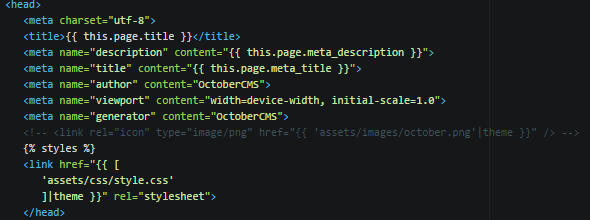
\includegraphics[width=\linewidth]{img/oc-layout-head.png}
  \caption{De 'head' structuur van de layout pagina}
  \label{fig:De 'head' structuur van de layout pagina}
\end{figure}

\noindent
Het meest interessante stukje code uit deze sectie zal de injectie van de CSS zijn. Stijlen kunnen rechtstreeks worden toegevoegd. Wanneer een stijl op een bepaalde pagina voorkomt, kan deze in de PHP sectie van de pagina worden geïmplementeerd. Een andere manier is gebruik te maken van Twig tags.

\begin{figure}[!ht]
  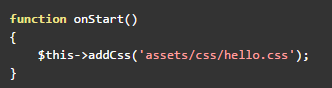
\includegraphics[width=75mm]{img/oc-styles-php.png}
  \centering
  \caption{Injectie van CSS via de onStart functie in de PHP sectie van de pagina.}
  \label{fig:CSS injectie via PHP code}
  \citep{BobkovAlexey2016OctoberCMSDocumentation}
\end{figure}

\begin{figure}[!ht]
  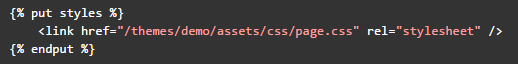
\includegraphics[width=100mm]{img/oc-styles-twig.png}
  \centering
  \caption{Injectie van CSS door gebruik te maken van Twig markup.}
  \label{fig:CSS injectie via Twig}
  \citep{BobkovAlexey2016OctoberCMSDocumentation}
\end{figure}

\pagebreak

\noindent
Verder onderscheiden we een navigatie die eerder al besproken is. Het actief zetten van een navigatie item is aan de hand van een IF-statement. Het controleert voor ieder menu item of het al dan niet de pagina's huidige ID is. Als dit het geval is, wordt de klasse 'active' toegevoegd. 

\begin{figure}[!ht]
  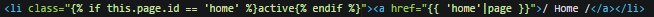
\includegraphics[width=\linewidth]{img/oc-layout-nav.png}
  \caption{If-statement om na te gaan of een menu item actief is.}
  \label{fig:Menu item actief test}
\end{figure}

\noindent
Binnen de 'main' sectie wordt de inhoud van de desbetreffende pagina ingeladen. Deze inhoud zal dus verschillend zijn voor elke pagina. Hoe deze inhoud geïmplementeerd wordt is zeer eenvoudig. In de configuratie sectie van iedere pagina is het mogelijk een template in te geven aan de hand van zijn document naam. Zo geef je voor elke gewenste pagina bijvoorbeeld default is als layout template. De pagina zal opgebouwd worden aan de hand van de default layout pagina. Inhoud van deze pagina wordt opgevuld daar waar de Twig tag 'page' staat. 

\begin{figure}[!ht]
  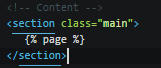
\includegraphics[width=50mm]{img/oc-layout-page.png}
  \centering
  \caption{De Twig tag zal vervangen worden door de inhoud van desbetreffende pagina.}
  \label{fig:Variabele pagina-inhoud.}
\end{figure}

\noindent
Bij de pagina footer wordt gebruik gemaakt van een partial. Zoals eerder werd besproken is dit een herbruikbaar stuk code die in een aparte file wordt bewaard. Het opdelen van code zorgt ervoor dat een pagina overzichtelijk blijft. 


\subsubsection{Aanmaken van een pagina met bijhorende plugin}
Er wordt slechts één proces doorlopen voor het aanmaken van een pagina met bijhorende plugin. De team pagina geeft een overzicht van de verschillende werknemers met bijgevoegde foto, naam, functie en aanwervingsjaar. Verder bevat de pagina een statische banner met een content block, die in de back-end via de browser kan worden aangepast door de eindgebruiker. 
\newline\newline
Het proces begint met het aanmaken van een plugin. Dit kan via verschillende manieren, hier werd geopteerd om de Builder plugin te gebruiken. Sommige stappen werden reeds via woord en beeld duidelijk gemaakt in vorig hoofdstuk, daarom zullen reeds aangehaalde stappen slechts kort besproken worden. 
\newline\newline
Begin met het aanmaken van een plugin door het een naam, auteur, beschrijving en icoon te geven. Vervolgens kan je voor de geselecteerde plugin een database tabel aanmaken. Iedere keer je de tabel gaat opslaan komt een pop-up venster tevoorschijn met genereerde query die uitgevoerd wordt op de database. Zo worden alle aanpassingen op deze tabel gedaan. 

\begin{figure}[!ht]
  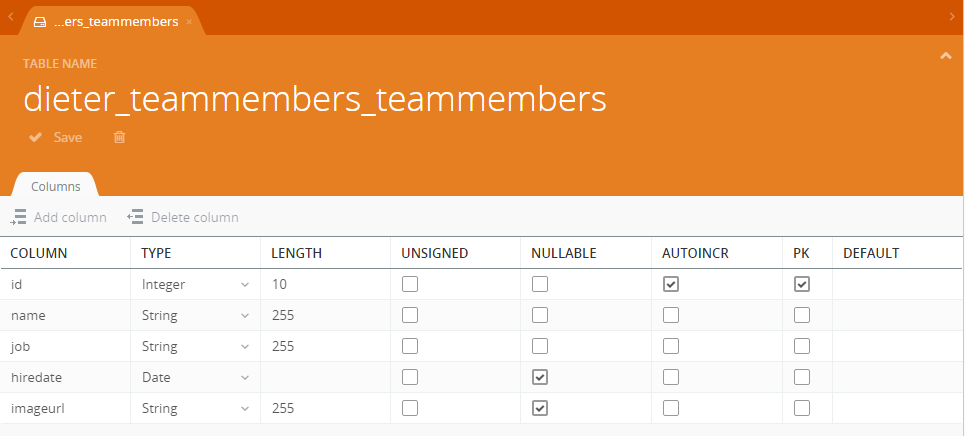
\includegraphics[width=\linewidth]{img/oc-plugin-teammember-db.png}
  \caption{Voeg de nodige rijen en vul de kolommen in waar nodig.}
  \label{fig:Teammember database tabel.}
\end{figure}

\noindent
De volgende stap is het aanmaken van de model klasse. Geef het model een naam en selecteer de database tabel. Het model is opgedeeld uit 'Form fields' en 'List fields'. De 'Form fields' of formuliervelden, zijn velden die weergegeven en geconfigureerd worden voor de invoer van nieuwe data. De 'List fields' of lijstvelden geven een overzicht van alle aangemaakte data weer in een lijst.
\newline\newline
Bij het aanmaken van de formuliervelden kan je allerhande velden toevoegen. Gaande van tekstvelden, dropdown velden tot file upload velden. Eenmaal een type geselecteerd kan de configuratie van dit veld gebeuren. Ieder veld heeft een 'Field name' die een naam krijgt gerelateerd aan de tabel. Andere velden zijn veelal verschillend, afhankelijk van het data type. De meeste velden spreken voor zich, zo niet zorgt het informatie icoontje voor bijhorende informatie. 

\begin{figure}[!ht]
  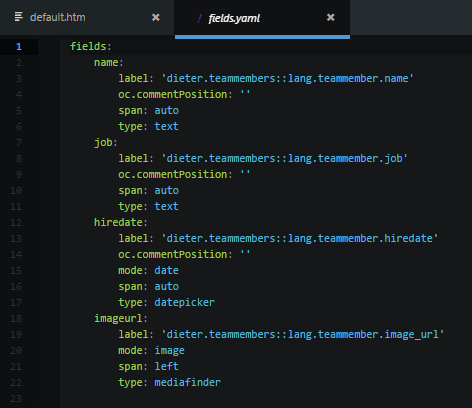
\includegraphics[width=100mm]{img/oc-plugin-model-fields.png}
  \centering
  \caption{De configuratie van alle velden is terug te vinden in de 'fields.yaml' file.}
  \label{fig:Teammember model fields.}
\end{figure}

\pagebreak
\noindent
De werking voor lijstvelden is gelijklopend met deze van de formuliervelden. 
Specifieke permissies werden niet toegevoegd, aangezien we slechts beschikken over één gebruiker.
\noindent
Maak nu een back-end menu item aan met een gepaste naam en icoon. De URL vullen we pas aan eenmaal de controller is aangemaakt. 
\newline\newline
We voegen een controller toe en geven hem een naam. We selecteren een model klasse als ook een menu item. Onder de 'Behaviors' tab selecteren we de checkboxen 'List- en Form controller behaviour'.
Deze opties zorgen voor de aanmaak van de standaard controller pagina's:  creëren, updaten, preview en overzicht.

\begin{figure}[!ht]
  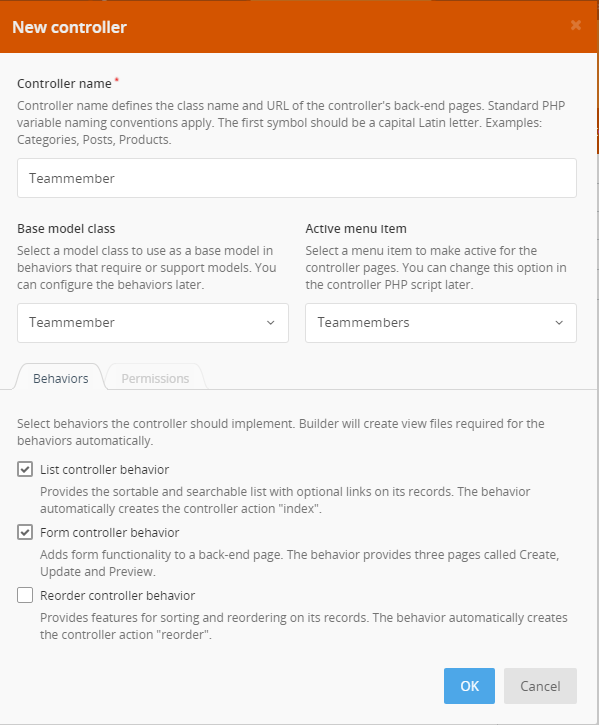
\includegraphics[width=100mm]{img/oc-plugin-teammember-controller.png}
  \centering
  \caption{Het pop-up venster voor de aanmaak van een controller.}
  \label{fig:Teammember controller pop-up.}
\end{figure}

\pagebreak

\noindent
Nu de controller is aangemaakt kunnen we de URL instellen bij het menu item. 
Dit waren de stappen bij het opstellen van een plugin via de Builder plugin. Hoewel dit een standaard configuratie van een plugin is, kan nu in code via een editor nog business logica worden toegevoegd. Er kunnen bijvoorbeeld nog aanpassingen volgen aan de modelklasse, controller klasse en eventuele toevoegingen van andere back-end pagina's.
\newline\newline
De team pagina heeft verder geen aanpassingen nodig, waardoor we rechtstreeks een front-end pagina kunnen aanmaken. Voeg een .htm file toe aan de 'pages' folder en vul de configuratie sectie in met naam, URL en Layout. De PHP sectie krijgt een onStart functie mee waarin we alle team leden gaan ophalen uit de database. 

\begin{minted}{c}
$this['members'] = Db::table('dieter_teammembers_teammembers')->get();
\end{minted}

\noindent
Het is nu mogelijk om de verzameling van leden te overlopen in de Twig sectie van de pagina. Overlopen van een collectie of verzameling doen we met een for-lus. 
Via de dot notatie (.) kunnen we een attribuut aanspreken van een teamlid. 

\begin{figure}[!ht]
  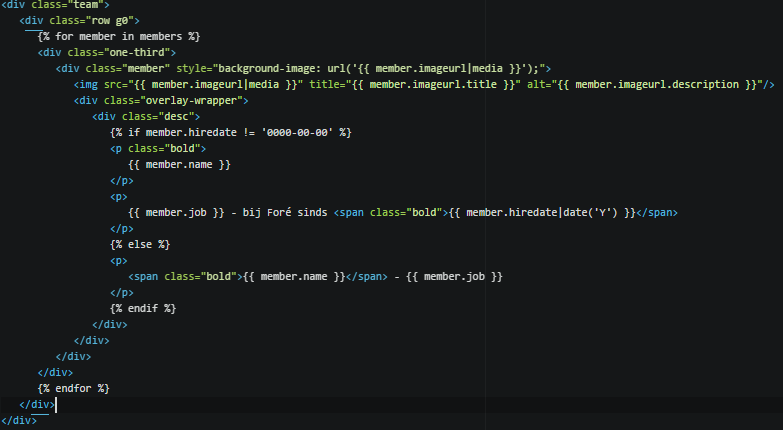
\includegraphics[width=\linewidth]{img/oc-plugin-teammember-page.png}
  \caption{Overloop de collectie via een for-lus}
  \label{fig:Teammember Front-end page.}
\end{figure}

\noindent
Bovenaan de pagina bevindt zich een banner met statische afbeelding en inhoud die aangevuld is via een content block. Het content block kan de eindgebruiker eenvoudig beheren via een teksteditor in de back-end van de browser.  

\begin{minted}{c}
  <div class="desc">
      
  </div>
\end{minted}

\begin{figure}[!ht]
  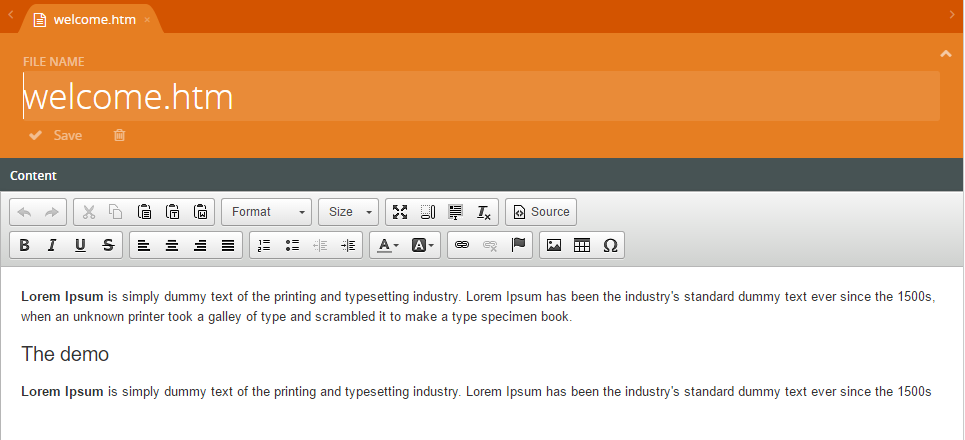
\includegraphics[width=\linewidth]{img/oc-contentblock.png}
  \caption{Eenvoudig tekst aanpassen via de browser, zonder enige technische kennis.}
  \label{fig:Teammember Content Block.}
\end{figure}

\pagebreak

\subsubsection{Beheersbaarheid van pagina's}
We zagen net dat het aanpassen van een content block heel eenvoudig in zijn werk gaat. We overlopen hier hoe we teamleden kunnen aanmaken en beheren. 
\newline\newline
Via het menu item 'Teammembers' in de taakbalk komen we op een overzicht met alle bestaande teamleden. Via de Create link komen we op de formulierpagina waar we eerder alle velden voor hebben ingesteld. We vullen een naam, job, aanwervingsdatum in en voegen een afbeelding toe via de Media Manager van OctoberCMS. Eenmaal opgeslagen wordt het nieuwe lid weergeven in de lijst. Een lid updaten kan door erop te klikken, aanpassingen door te voeren en terug op te slaan. 
\newline\newline
Er is een mogelijkheid om pages, partials, layouts en components aan te passen via de browser, toch is dit iets dat je beter aanpast via een editor en eerder verborgen staat voor de eindgebruiker. 